\begin{frame}
\frametitle{ Planning }
\tiny{\textcolor{blue} {We have considered FlexRay architecture\footnote{\tiny{\textcolor{blue}{Florian Sagstetter,
               Martin Lukasiewycz and
               Samarjit Chakraborty, Generalized Asynchronous Time-Triggered Scheduling for FlexRay, {IEEE} Trans. on {CAD} of Integrated Circuits and Systems}}} to explain our idea.
FlexRay demonstrates how a communication protocol can work in 
automotive domain with high data rates.The architecture is given below:}}

\begin{figure}
\begin{center}
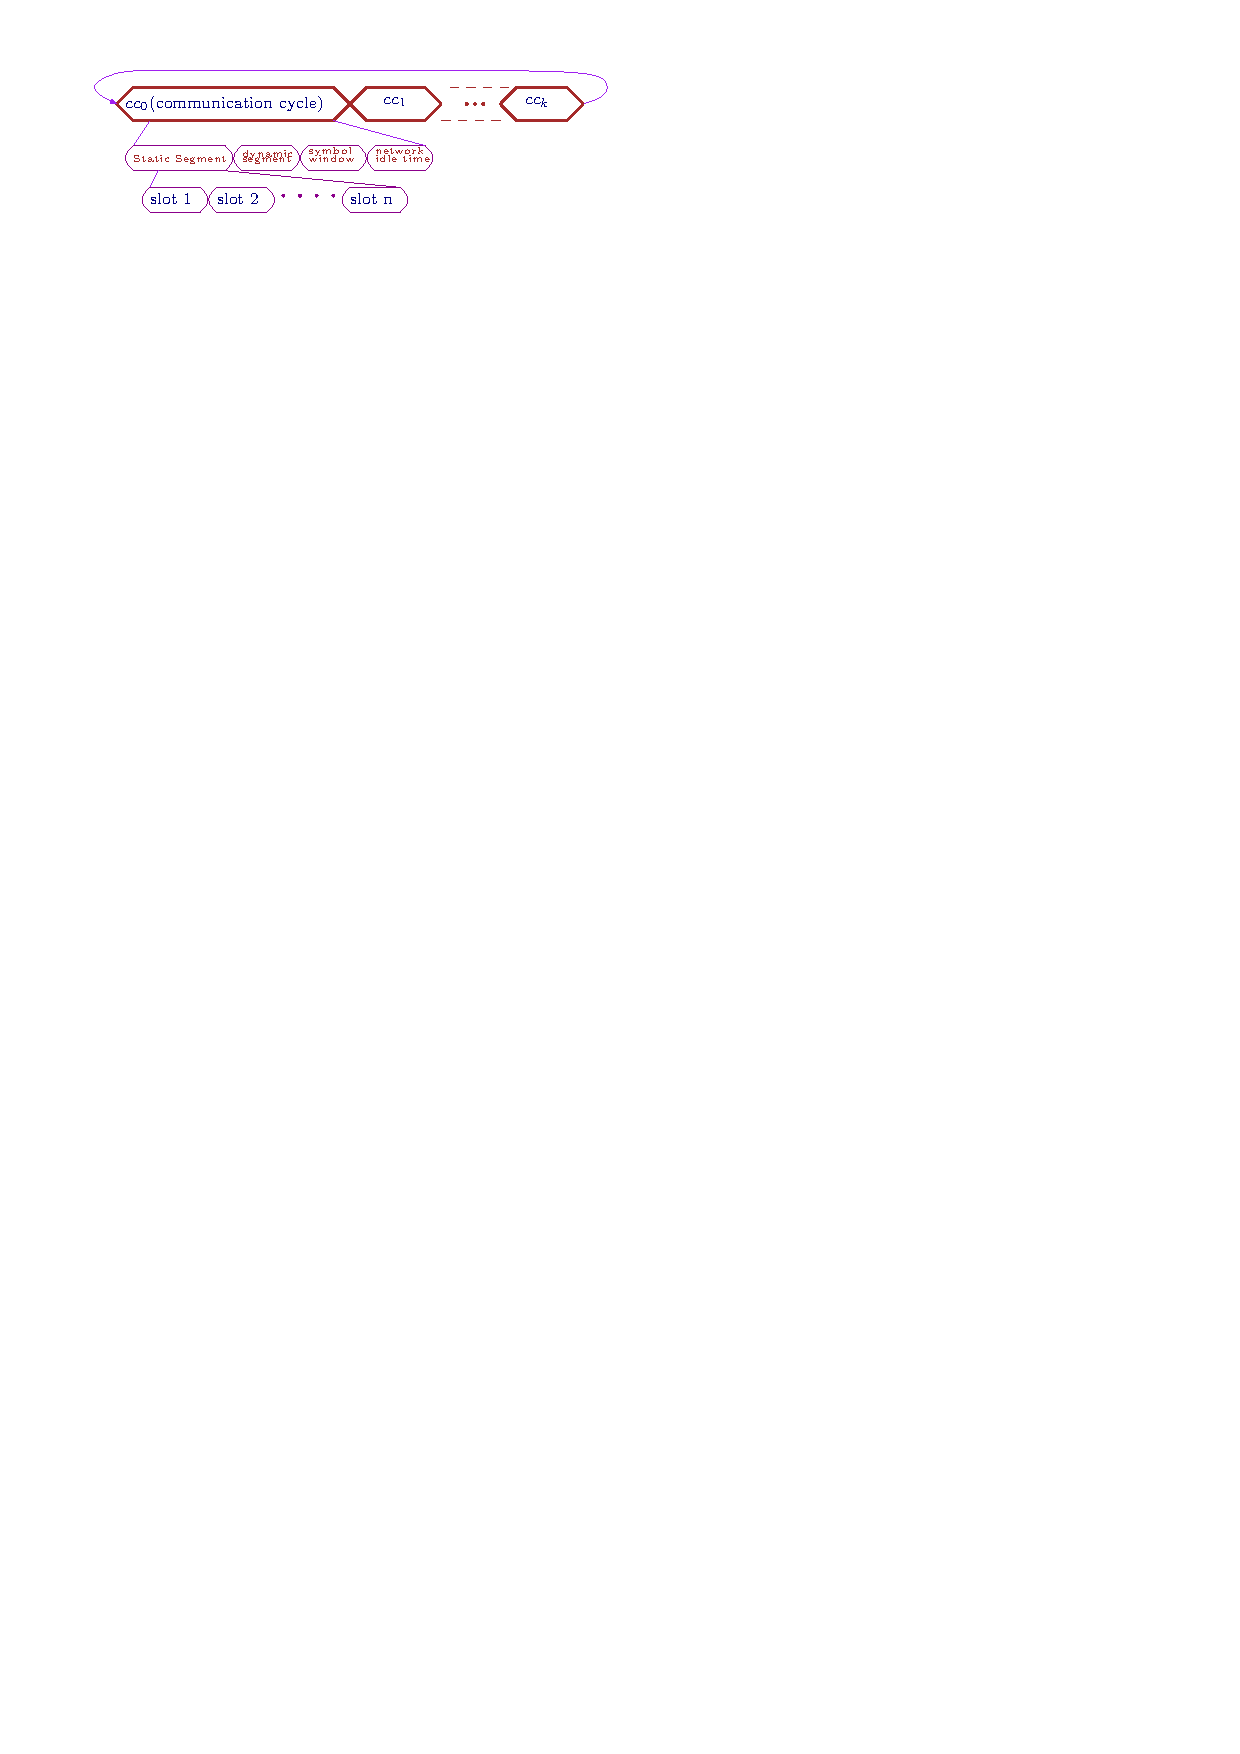
\includegraphics[width=55mm]{Flex_Ray.pdf}
\end{center}
%\vspace{-0.1in}
\caption{{\em \tiny{\textcolor{blue}{Basic  structure of FlexRay illustrating communication cycles}}}} \label{fig1}
\end{figure}

\begin{itemize}
 \item \tiny{\textcolor{blue}{FlexRay schedule is organised in multiple  repeating communication cycles}}
 \item \tiny{\textcolor{blue}{Each cycle is divided into $4$ different segments}}
        \begin{itemize}
              \item \tiny{\textcolor{blue} {Static segment}}
              \item \tiny{\textcolor{blue} {Dynamic segment}}
              \item \tiny{\textcolor{blue} {Symbol window}}
              \item \tiny{\textcolor{blue} {Network idle time}}
        \end{itemize}
        
\item \tiny{\textcolor{blue}{WE are here only considering static segment:}}
      \begin{itemize}
       \item \tiny{\textcolor{blue}{Consists of fixed number slots with equal size}}
       \item \tiny{\textcolor{blue}{Time-triggered static segment used for scheduling}}
      \end{itemize}

 
       
\end{itemize}

\end{frame}